\documentclass[crop,tikz,12pt]{standalone}

\usetikzlibrary{arrows.meta}

\colorlet{mygrey}{white!35!black}

\begin{document}

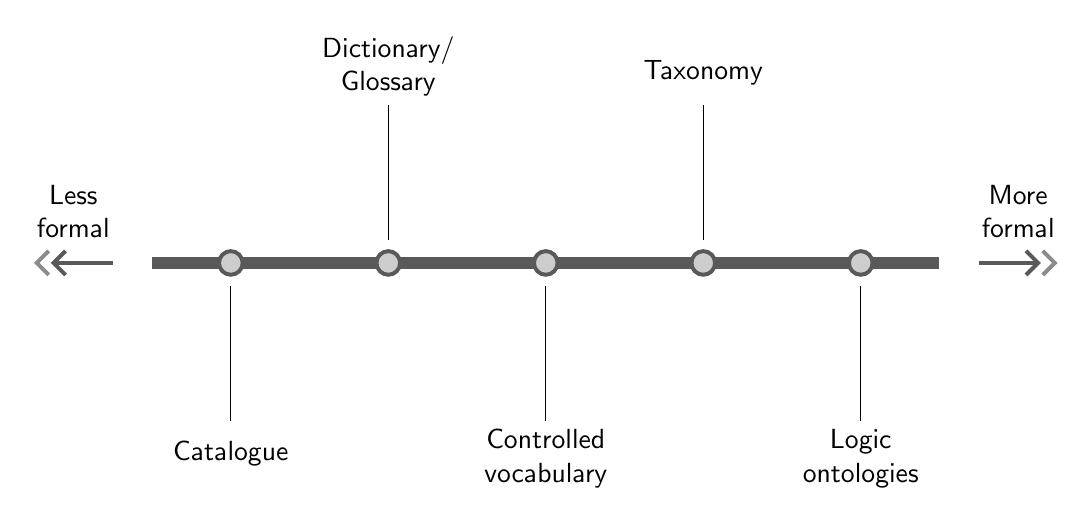
\begin{tikzpicture}[
    every node/.style={font=\sffamily},
    spectrum/.style={line width=1.5mm,draw=mygrey},
    arrow/.style={line width=0},
    vocab north/.style={minimum height=2\baselineskip,anchor=south,align=center},
    vocab south/.style={minimum height=2\baselineskip,anchor=north,align=center},
    dot/.style={fill=mygrey!30!white,line width=0.5mm,draw=mygrey}
]

\node [anchor=south,align=center] at (-2, 2mm) {Less\\formal};
\draw [{Straight Barb[color=mygrey!70!white] . Straight Barb[]}-,color=mygrey,line width=0.5mm] (-2.5,0) -- (-1.5, 0);

\node [anchor=south,align=center] at (10, 2mm) {More\\formal};
\draw [-{Straight Barb[] . Straight Barb[color=mygrey!70!white]},color=mygrey,line width=0.5mm] (9.5,0) -- (10.5, 0);



\draw [spectrum] (-1,0) -- (9,0);

\filldraw [dot] (0, 0) circle (1.5mm);
\draw [arrow] (0, -2) node [vocab south] {Catalogue} -- (0, -3mm);

\filldraw [dot] (2, 0) circle (1.5mm);
\draw [arrow] (2, 2)  node [vocab north] {Dictionary/\\Glossary} -- (2, 3mm);

\filldraw [dot] (4, 0) circle (1.5mm);
\draw [arrow] (4, -2) node [vocab south] {Controlled\\vocabulary} -- (4, -3mm);

\filldraw [dot] (6, 0) circle (1.5mm);
\draw [arrow] (6, 2)  node [vocab north] {Taxonomy} -- (6, 3mm);

\filldraw [dot] (8, 0) circle (1.5mm);
\draw [arrow] (8, -2) node [vocab south] {Logic\\ontologies} -- (8, -3mm);


\end{tikzpicture}

\end{document}
